\documentclass[tikz,border=5mm]{standalone}
\usetikzlibrary{calc}
\begin{document}
	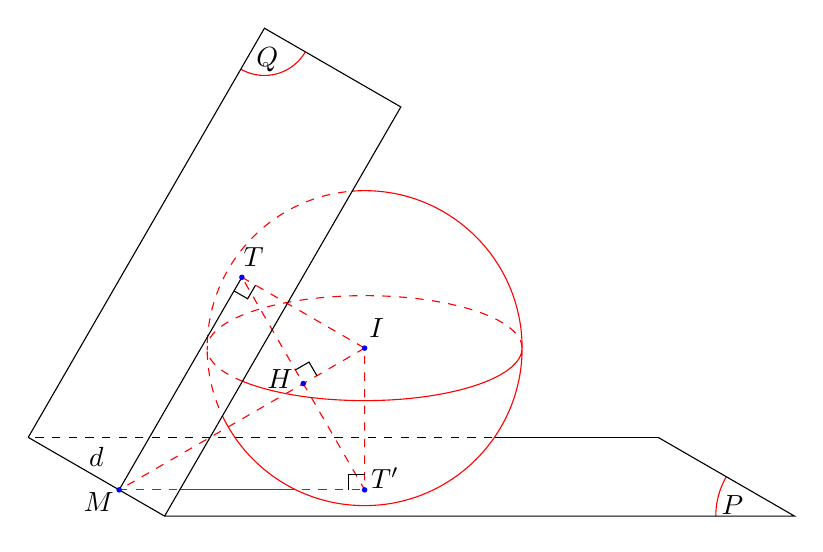
\begin{tikzpicture}[>=stealth]
		\def\vugoc(#1,#2,#3)(#4){
			\draw ($(#2)!#4!(#1)$)--($($(#2)!#4!(#1)$)+($(#2)!#4!(#3)$)-(#2)$)--($(#2)!#4!(#3)$)}
		\def\r{2}
		\pgfmathsetmacro{\rm}{0.9*\r}
		\pgfmathsetmacro{\h}{2*\rm *sin(30)}
		\path
		(0:0) coordinate (I)
		(-150:2*\rm) coordinate (M)
		(270:\h) coordinate (T')
		(150:\h) coordinate (T)
		(0:\r) coordinate (A)
		(180:\r) coordinate (B)
		(intersection of T--T' and M--I) coordinate (H)
		($(M)+(150:2*\r/3)$) coordinate (C1)
		($(M)+(-30:\r/3)$) coordinate (C2)
		($(C2)+(0:4*\r)$) coordinate (C3)
		($(C1)+(0:4*\r)$) coordinate (C4)
		($(C2)+(60:3*\r)$) coordinate (C5)
		($(C1)+(60:3*\r)$) coordinate (C6)
		;
		\begin{scope}
			\clip (I) circle (\r);
			\draw[dashed,red](M)--(T');
			\draw[dashed] (C4)--(C1);
		\end{scope}
		\begin{scope}
			\clip (C1)--(C2)--(C5)--(C6)--cycle;
			\draw[dashed,red](M)--(T');
			\draw[dashed] (C4)--(C1);
		\end{scope}
		\begin{scope}
			\clip (270:\r) arc (-90:-150:\r)--(C5)--(C2)--(C3)--(C4)--cycle;
			\draw[red] (M)--(T');
			\draw[dashed](C4)--(C1);
		\end{scope}
		\begin{scope}
			\clip (A) arc (0:-90:\r)--(C3)--(C4)--cycle;
			\draw (C4)--(C1);
		\end{scope}
		\begin{scope}
			\clip (C1)--(C2)--(C3)--(C4)--cycle;
			\draw[red] (C3) circle (10mm);
		\end{scope}
		\begin{scope}
			\clip (C1)--(C2)--(C5)--(C6)--cycle;
			\draw[red] (C6) circle (6mm);
		\end{scope}
		\draw[dashed,red] (A) arc (0:180:{\r} and {\r/3})
		(T)--(I)--(T')--cycle (I)--(M);
		\begin{scope}
			\clip (C2)--(C3)--(C5)--cycle;
			\draw[red] (0:0) circle (\r) (0:\r) arc (0:-180:{\r} and {\r/3});
		\end{scope}
		\begin{scope}
			\clip (C1)--(C2)--(C5)--(C6)--cycle;
			\draw[red,dashed] (0:0) circle (\r) (0:\r) arc (0:-180:{\r} and {\r/3});
		\end{scope}
		\draw (C1)--(C2)--(C3)--(C4) (C2)--(C5)--(C6)--(C1)
		(T)--(M);
		\vugoc(M,T,I)(2mm);
		\vugoc(M,T',I)(2mm);
		\vugoc(T,H,I)(2mm);
		\foreach \x in {M,T,T',H,I}{\fill[blue] (\x) circle (1pt);}
		\foreach \x/\i in {M/210,T/60,I/60,T'/30,H/170}{\path ($(\x)+(\i:3mm)$)node{$\x$};}
		\path
		($(C3)+(170:8mm)$) node{$P$}
		($(C6)+(275:4mm)$) node{$Q$}
		(C1)--(C2)node[midway,above]{$d$}
		;
	\end{tikzpicture}
\end{document}